\documentclass[xcolor=table, aspectratio=169]{beamer}
%\usepackage{arev}
\usepackage{amsmath,amssymb,amscd}
\usepackage{dsfont}
\usepackage{mathrsfs}
\usepackage{yfonts}
\usepackage{bm}
\usepackage{graphicx}
\usepackage{tabularx}
\usepackage{animate}
\usepackage{listings}
%\usepackage{mathtools}
%\usepackage{ifthen}

\usepackage{xeCJK}
\usepackage{fontspec}
\usepackage{inter}
%\usepackage{unicode-math}
\usefonttheme{professionalfonts}
\usefonttheme[onlymath]{serif}
%\setmathfont{Latin Modern Math}
\setCJKmainfont{Noto Sans CJK SC}
%\setCJKmainfont{FZXiHeiI-Z08}
\newcolumntype{x}{>{\centering\arraybackslash}X}
\renewcommand{\arraystretch}{1.5}
\DeclareMathOperator{\img}{img}
\DeclareMathOperator{\hhom}{Hom}
\DeclareMathOperator{\id}{id}
\DeclareMathOperator{\sspan}{span}
\usepackage{tikz}
	\usetikzlibrary{calc}
	\usetikzlibrary{arrows,shapes, positioning, matrix}
	\usetikzlibrary{decorations.markings}
	\tikzset{>=stealth}
	\tikzstyle arrowstyle=[scale=1]
	\tikzstyle directed=[postaction={decorate,decoration={markings,
 	   mark=at position .15 with {\arrow[arrowstyle]{stealth}}}}]
\tikzstyle string=[thick,postaction={decorate,decoration={markings,
    mark=at position .55 with {\arrow[arrowstyle]{stealth}}}}]
\tikzstyle dual_string=[dashed,postaction={decorate,decoration={markings,
    mark=at position .55 with {\arrow[arrowstyle]{stealth}}}}]

\tikzstyle dw=[thick,postaction={decorate,decoration={markings,
    mark=at position 1 with {\arrow[arrowstyle]{stealth}}}}]
\tikzstyle group=[mbg]
\newcommand*{\halfway}{0.5*\pgfdecoratedpathlength+.5*8pt}\tikzstyle arrowstyle=[scale=1]
\newcommand*{\halfwayb}{0.5*\pgfdecoratedpathlength}
\tikzstyle arrowstyle=[scale=1]
\tikzstyle fermion=[thick,postaction={decorate},decoration={markings,
    mark=at position \halfway with {\arrow[arrowstyle]{latex}}}]
\tikzstyle fermion2=[thick,postaction={decorate},decoration={markings,
        mark=at position \halfwayb with {\arrow[arrowstyle]{latex}}}]
\usepackage{tikz-cd}
\usepackage{pgffor}

\DeclareMathOperator{\tr}{Tr}
\DeclareMathOperator{\im}{Im}
\DeclareMathOperator{\re}{Re}

\mode<presentation>
{
  %\usetheme{Warsaw}
  % or ...
  %\useoutertheme{rectangle}
  \setbeamertemplate{frametitle}[default][center]
  \defbeamertemplate{itemize item}{flat}{\begin{pgfpicture}{-1ex}{0ex}{1ex}{2ex}
      \pgfpathcircle{\pgfpoint{0pt}{.6ex}}{0.6ex}
      \pgfusepath{fill}
    \end{pgfpicture}%
  }
  \defbeamertemplate{itemize subitem}{flat}{\footnotesize\raise0.5pt\hbox{\textbullet}}
  \defbeamertemplate{itemize subsubitem}{flat}{\footnotesize\raise0.5pt\hbox{\textbullet}}

  %\useinnertheme{circles}
  \setbeamertemplate{items}[flat]
  \setbeamertemplate{sections/subsections in toc}[circle]
  \setbeamertemplate{blocks}[rounded]
  \setbeamertemplate{title page}[default][colsep=-4bp,rounded=true]
  \setbeamertemplate{part page}[default][colsep=-4bp,rounded=true]
  \setbeamercovered{transparent}
  %\usecolortheme{spruce}
  %\definecolor{THU}{RGB}{116,61,130}
  \definecolor{mbg}{RGB}{0,0,160}
  \setbeamercolor*{palette primary}{fg=white,bg=mbg}
  \setbeamercolor*{titlelike}{parent=palette primary}
  \setbeamercolor*{structure}{fg=mbg}
  \setbeamercolor{frametitle}{fg=white,bg=mbg}
  % or whatever (possibly just delete it)
  \setbeamercolor{block title}{bg=mbg,fg=white}
  \setbeamercolor{block body}{bg=mbg!15}


  \addtobeamertemplate{navigation symbols}{}{ \hspace{1em}%
    \usebeamerfont{footline}%
    \insertframenumber / \inserttotalframenumber }
}


%\usepackage[english]{babel}
% or whatever

%\usepackage[latin1]{inputenc}
% or whatever

%\usepackage{times}
%\usepackage[T1]{fontenc}
% Or whatever. Note that the encoding and the font should match. If T1
% does not look nice, try deleting the line with the fontenc.

\title[NGA Bootstrap] % (optional, use only with long paper titles)
{Nullspace-Guided Adaptive Bootstrap for \\Quantum Many-body Systems}

\author[Y Qi] % (optional, use only with lots of authors)
{戚~扬}
% - Give the names in the same order as the appear in the paper.
% - Use the \inst{?} command only if the authors have different
%   affiliation.

\institute[Fudan] % (optional, but mostly needed)
{复旦大学物理学系}
% - Use the \inst command only if there are several affiliations.
% - Keep it simple, no one is interested in your street address.

\date{第六届量子物质新前沿会议, 昆明 2026}
% - Either use conference name or its abbreviation.
% - Not really informative to the audience, more for people (including
%   yourself) who are reading the slides online

\subject{Theoretical Physics}
% This is only inserted into the PDF information catalog. Can be left
% out.




% If you have a file called "university-logo-filename.xxx", where xxx
% is a graphic format that can be processed by latex or pdflatex,
% resp., then you can add a logo as follows:

\pgfdeclareimage[height=1cm]{university-logo}{../resources/fudan}
\logo{\pgfuseimage{university-logo}}

\AtBeginSection[]
{
  \begin{frame}<beamer>{Outline}
    \tableofcontents[currentsection,currentsubsection]
  \end{frame}
}


% Delete this, if you do not want the table of contents to pop up at
% the beginning of each subsection:

\begin{document}

\begin{frame}
  \titlepage
\end{frame}

\begin{frame}{Collaborators}
  \begin{itemize}
    \item Xu-Cheng Wang (王勖成), Fudan University.
    \begin{center}
      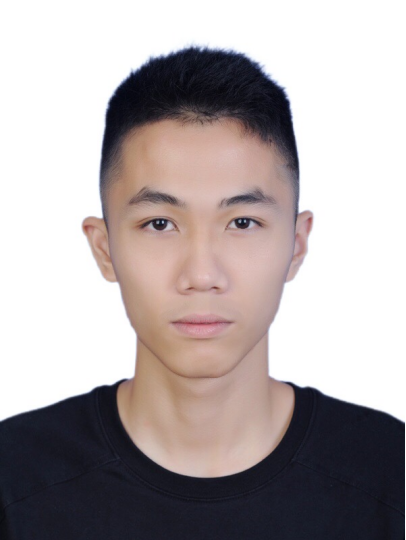
\includegraphics[height=3cm]{../people/xuchengwang}
    \end{center}
  \item Xu-Cheng Wang and Yang Qi, arXiv:2608.xxxxx
  \item \url{https://github.com/JefferyWangSH/QMBBoot-NGA}
  \end{itemize}
  % \[E=mc^2.\]
\end{frame}

\section{Introduction: Quantum Many-body Bootstrap}

\begin{frame}{Example: SHO}
  Consider a simple harmonic oscillator:
  \[H=\frac12p^2+\frac12x^2.\]
  \begin{itemize}
  \item Classically: $\langle H\rangle\geq 0$, $\langle H\rangle=0$ when $\langle x\rangle=\langle p\rangle = 0$.
  \item QM: $\Delta x\cdot \Delta p\geq\hbar$, $\langle H\rangle\geq \frac12\hbar$.
  \end{itemize}
  \begin{columns}
    \column{.5\textwidth}
    \begin{block}{Formal proof.}<2->
      \[\langle (p+ix)(p-ix)\rangle\geq 0.\]
      \[\langle p^2\rangle+\langle x^2\rangle\geq -i\langle [x,p]\rangle =\hbar.\]
      \[\therefore \langle H\rangle\geq \frac\hbar2.\]
    \end{block}
    \column{.4\textwidth}
    % \begin{block}{Essential factors}
    Essential factors:
      \begin{itemize}
      \item<3-> $\langle O^\dagger O\rangle \geq 0.$
      \item<4-> Commutation relation.
      \item<5-> Minimize $\langle H\rangle$.
      \end{itemize}
    %\end{block}
  \end{columns}
\end{frame}

\begin{frame}{Bootstrap algorithm}

  \begin{columns}
    \column{.4\textwidth}
    \begin{block}{Minimization problem}
      \begin{align*}
        E=\min_{f} \quad &\langle H\rangle,\\
        \mathrm{s.t.} \quad &\langle O^\dagger O\rangle \geq 0.
      \end{align*}
      where $f: O\mapsto\langle O\rangle$.
    \end{block}

    % \begin{center}
    \centering\includegraphics{relax-method}
    %\end{center}
    \column{.6\textwidth}
    Bootstrap is a relaxation method:
    \begin{itemize}
    \item Givens \textbf{lower bound} of the ground-state energy.
    \item \textbf{Compliments} instead of \textbf{competes} with variational method such as DMRG.
    \item Together with DMRG, can give \textbf{rigorous bounds} to the ground-state energy and other observables.
    \end{itemize}
  \end{columns}
  
\end{frame}

\begin{frame}{Bootstrap algorithm}

  \begin{columns}
    \column{.5\textwidth}
    \begin{block}{Ideal minimization problem}
      \begin{align*}
        E=\min \quad &\langle H\rangle,\\
        \mathrm{s.t.} \quad &\langle O^\dagger O\rangle \geq 0.
      \end{align*}
    \end{block}
    \begin{block}{Truncation}
      \begin{itemize}
      \item A set of basis: $O_i, i=1,\ldots,N$; $\mathcal V=\sspan\{O_i\}$.
      \item $\mathcal M:=\mathcal V^\dagger\mathcal V$.
      \item $\bm x\in \mathcal M^\ast$: a functional $O\mapsto \langle O\rangle$.
      \item $M(\bm x)$: a $N\times N$ matrix $M_{ij}:=\langle O_i^\dagger O_j\rangle.$
      \end{itemize}
    \end{block}
    \column{.5\textwidth}

  \end{columns}
  
\end{frame}

\begin{frame}{Bootstrap algorithm}

  \begin{columns}
    \column{.5\textwidth}
    Ideal minimization problem:
    \begin{align*}
      E=\min \quad &\langle H\rangle,\\
      \mathrm{s.t.} \quad &\langle O^\dagger O\rangle \geq 0; \langle 1\rangle=1.
    \end{align*}
    Truncation:
    \begin{itemize}
    \item A set of basis: $O_i, i=1,\ldots,N$; $\mathcal V=\sspan\{O_i\}$.
    \item $\mathcal M:=\mathcal V^\dagger\mathcal V$.
    \item $\bm x\in \mathcal M^\ast$: a functional $O\mapsto \langle O\rangle$.
    \item $M(\bm x)$: a $N\times N$ matrix $M_{ij}:=\langle O_i^\dagger O_j\rangle.$
    \end{itemize}
    Truncated min problem:
    \begin{align*}
      E=\min \quad & \bm c^T\bm x,\\
      \mathrm{s.t.}\quad & M \geq 0; A\bm x=\bm b.
    \end{align*}
    \column{.5\textwidth}
    
  \end{columns}
  
\end{frame}

\section{Method: Nullspace-Guided Adaptive (NGA) Bootstrap}

\section{Results: Application to 1d Hubbard Model}

\section{Conclusion and future directions}

\end{document}

%%% Local Variables:
%%% mode: latex
%%% TeX-engine: xetex
%%% End:
